%!TEX root = ../thesis.tex
%*******************************************************************************
%****************************** Second Chapter *********************************
%*******************************************************************************

\chapter{Results of Physical Properties Modification in Novel 2D materials \label{chap:5}}

\ifpdf
    \graphicspath{{Chapter5/Figs/Raster/}{Chapter5/Figs/PDF/}{Chapter5/Figs/}{Chapter5/Figs/Vector/}}
\else
    \graphicspath{{Chapter5/Figs/Vector/}{Chapter5/Figs/}}
\fi

This is the second part of the results of the thesis. Here we will discuss some of the possible ways to modify the physical properties of 2D materials. As before, each section will be focused on an unique way to change the properties of materials, namely number of layers, mechanical strain, adatom adsorption, heterostructure and defect induction. In consist with the theme of the thesis, which is about novel 2D materials, we will continue to introduce other new 2D that has been discovered and whose properties will be modified. Some of the studies here are the continuum of the works in the previous chapter where properties are determined only, here those properties will be modified. 


\section{Number of layers}
\subsection[Few-layer of Calcium hydroxide]{Few-layer of Calcium hydroxide \footcite[This work is published in:][]{Aierken2015.porlandite}}

We have seen several monolayer systems that exacted from layered materials such 2D-BN, 2D-MoS$_2$, in this work, we further explore this process for alkaline earth metal hydroxides (AEMHs), which pose a layered structure in the bulk form. It was exfoliated  to few-layer, the experiment and the theoretical modelling is reported in this section. In contrast to the abundant literature on graphenelike ultra-thin structures, few-layer AEMHs have not been investigated so far. Bulk forms of AEMHs are layered structures belonging to the $P\overline{3}m1$ space group\cite{structure1} and the crystal structure of a layered AEMHs comprises stacked sheets of MO$_6$ (M=alkaline earth metals) edge-sharing octahedra, see \autoref{fig:str_caoh2}. At each corner of an octahedron, each O atom binds one H atom and the latter interacts with three neighboring hydroxyl groups of the adjacent layer. Early studies on bulk AEMHs revealed that the application of temperature and pressure may result in dramatical changes in their crystal structure and their electronic properties\cite{amorphization1,amorphization2,amorphization3,amorphization4,transition1,transition2,transition3,transition4} . Moreover, early theoretical studies showed the reliability of the use of first principle calculations with a plane-waves basis set in combination with the generalized gradient approximation exchange-correlation functional for the investigation of structural and electronic properties of these materials\cite{Winkler1995,Baranek2001,Azuma2011,DArco1993}.

\begin{figure}
\centering
\includegraphics[width=0.8\textwidth]{str_caoh2.eps}
\caption{\label{fig:str_caoh2} Atomic structure of bulk Ca(OH)$_2$: (a)
tilted view, (b) top view of one layer. }
\end{figure}

Although the structural and electronic properties of bulk AEMHs have been
investigated before \cite{Azuma2011,Pishtshev,Pishtshev1} , single layers of 
these materials have never been studied before and their stability is 
still an open question. However, advances 
in experimental techniques made exfoliation and growth of such 
structures possible\cite{new1,new2}. Especially the Portlandite material, Ca(OH)$_2$,
which has been the 
main product of hydration of Portland cement, CaO, is one of the most well-known 
AEHMs, characteristic properties of ultra-thin structures of Portlandite have 
not been reported yet. In this study we investigate, both experimentally and theoretically, 
the structural, electronic, magnetic, vibrational and mechanical 
characteristics of bulk, bilayer and monolayer Ca(OH)$_{2}$ and discuss how these properties change with the number of layers.  Particularly, the result of the phonon calculation is presented for the confirmation of the stability of the newly proposed 2D material.

To assess the mechanical strength of the material, in addition to the elastic moduli that we have introduced in \autoref{chap:3}, here we calculate another useful parameter that closely related to the Young's modulus, which is called the in-plane stiffness of the materials. We 
focused on the harmonic range of the elastic deformation, where the structure 
responded linearly to strain $\epsilon$. The stretching of the Ca(OH)$_{2}$ is 
achieved by increasing the equilibrium lattice constant a$_{0}$ by $\Delta$a, 
to attain the axial strain $\epsilon$ = $\Delta$a/a$_{0}$. We optimized the 
atomic structure at each increment of the strain, $\Delta\epsilon$ =0.01 and 
calculated the total energy under strain E$_{T}$($\epsilon$). Then the strain 
energy can be given by, E$_{S}$ = E$_{T}$($\epsilon$) - E$_{T}$($\epsilon$=0); 
namely, the total energy at a given strain $\epsilon$ minus the total energy at 
zero strain. Then, using the following formula, one can calculate the in-plane 
stiffness. 

\begin{equation}
 C = (\dfrac{1}{A_{0}})(\dfrac{d^{2}E_{S}}{d\epsilon^{2}}),
\end{equation}
where A$_{0}$ is the equilibrium area of the supercell.

As explained in detail in the following sections, unitcells including one Ca,
two O and two H are the primitive cells of both monolayer and bulk structures, 
it is doubled for bilayer. Cohesive energy per unit cell,
$E_{coh}$ is presented in \autoref{tab:str2_caoh2} and is calculated according to the formula:
$E_{coh}=E_{tot}-nE_{Ca}-2nE_O-2nE_H$, where $E_{tot}$ is the total energy
of the unit cell of Ca(OH)$_2$, $E_X$ is the single atom total energy of atom $X$
and $n$ is the number of Ca atoms for the corresponding unit cell, i.e.
$n=1$, $n=2$ and $n=1$ for monolayer, bilayer and bulk, respectively. 

\subsubsection{Computational details}

\begin{footnotesize}
\begin{description}
\item[Simulation program:] VASP and PHON\cite{alfe}
\item[Energy cut-off:] 500 eV
\item[Pseudopotentials:] PBE-GGA(PAW)
\item[k points (Monkhorst-Pack):] 35$\times$35$\times$1 and 25$\times$25$\times$11 for few-layer and bulk Ca(OH)$_{2}$, respectively 
\item[Vacuum:] 25~\AA
\item[Energy and force convergence criterion:] 10$^{-5}$ eV and 10$^{-2}$ eV/\AA, respectively
\item[vdW corrections:] DFT-D2 method of Grimme \cite{Grimme}
\item[Charge analysis:] Bader's charge analysis method\cite{Bader1,Bader2,Bader3}
\end{description}
\end{footnotesize}



\subsubsection{Experimental measurements}


Before our theoretical investigation of few-layer Ca(OH)$_{2}$, first we 
present the experimental realization and detailed theoretical analysis of the
characteristics of bulk Ca(OH)$_{2}$ crystals.


\begin{figure}[htbp]
\centering
\includegraphics[width=8.5cm]{exp_caoh2.eps}
\caption{\label{fig:exp_caoh2} (a) Optical image of the crystal structure and (b) Raman 
spectrum measured using 488 nm laser in the low and the high frequency region. 
The fundamental phonon branches located at the low frequency (100-400 cm$^{-1}$  range) and the high frequency (~3620 cm$^{-1}$) are associated with the OH  stretching mode. (c) XRD measurements}
\end{figure}

Ca(OH)$_{2}$ crystals were grown using the hydrolysis technique by using 
Ca$_{3}$SiO$_{5}$ micro-pallets. Ca$_{3}$SiO$_{5}$ was mixed at different water 
to solid ratios ranging from 0.2 to 0.9 by molar weight. The mixture was heated 
up to 40 $^{\circ}\mathrm{C}$ in a controlled reaction chamber for 3 hours and 
controllably cooled down to 5 $^{\circ}\mathrm{C}$ for 24 hours using a
temperature controller. The growth time depends on the total water to solid 
ratio as well as the growth temperature. Growth time was around 8 hours for 0.6 
water to solid ratio and 40 $^{\circ}\mathrm{C}$ growth temperature. 
Longer growth time typically resulted in a dendritic morphology where the 
growth was mostly in the c-axis direction. Synthesized crystals displayed rather sharp (FWHM ~ 7 cm$^{-1}$) Raman feature at 280 cm$^{-1}$ and our XRD measurements displayed sharp (00l) reflections at 19.1, 39, 56.2, 77.7 degrees implying that crystals have lamellar nature.  
 

Synthesized crystals were around 0.1-2 mm in size and they 
were filtered from the solution. After the filtering process, crystallites were 
washed off using 18.2 MOhm.cm DI wafer multiple times and dried under inert Ar 
gas. Crystallites were exfoliated using micro-mechanical exfoliation technique 
onto thermal silicon oxide / Si substrates. We find that the contrast 
was improved for an oxide thickness around 265-285 nm.
Exfoliated flakes displayed rather sharp edges (see \autoref{fig:exp_caoh2}) with 
well-defined angles of 120\textdegree ~and 60\textdegree ~implying that the 
materials are highly crystalline. Interestingly, synthesized Ca(OH)$_{2}$ flakes 
are layered in agreement with theoretical calculations and these flakes can be 
easily exfoliated using the Scotch tape technique on different substrates. 
The exfoliated flakes do not show any signs of structural imperfection, pit 
formation, and overall rather flat surfaces can be obtained. In \autoref{fig:exp_caoh2}, the 
yellowish looking regions actually correspond to regions where the thickness is 
around 50-100 nm (50-100 layers) while the blue features are only 10-50 nm in 
thickness. Considering the ease to exfoliate this material, experimentally and 
theoretically we predict that they can be eventually isolated down to mono- and 
few-layers on various substrates.

In addition, micro-Raman measurements were performed using a 488 nm laser on a 
2 micron square spot using a high intensity laser of 10 mW. We noticed that 
few-layers of Ca(OH)$_{2}$ were not subject to local over-heating / 
decomposition effects unlike transition metal dichalcogenides (MoS$_2$, 
WS$_2$, etc.) which typically decompose around 100 microWatt power using a 
similar laser excitation spot. We attribute this to the low absorption of the 
material associated with the rather large band gap. Raman measurements 
displayed various peaks in the 100-1000 cm$^{-1}$ range. The high frequency peak 
at 3620 cm$^{-1}$ is associated with the O-H stretching mode $A_{1g}$. In 
addition, the low frequency $E_u(T)$ mode is found at 280 cm$^{-1}$.  

Here, we note that even though this material is a direct gap semiconductor, 
their band gap is well beyond our detectors range and since the insulators 
cannot be excited with such high laser wavelength, PL measurements are 
virtually impossible.

\subsubsection{Structure properties of C\lowercase{a}(OH)$_{2}$}\label{strcuture}

The bulk structure of Portlandite is formed by the stacking of individual Ca(OH)$_2$ monolayers on top of each other, see \autoref{fig:str_caoh2}. As we will exam and discuss the stacking in detail in the following paragraphs, we learned that the AA stacking is the ground state atomic configuration for bulk and multilayer structures of Ca(OH)$_2$. In \autoref{tab:str_caoh2}, optimized lattice parameters of the bulk structure together with experiments and other theoretical calculation are presented. Our results consist with reference \cite{Pishtshev} and together they have good agreement with experiments. This justify the reliability of our calculations. 

In the 5-atomic hexagonal primitive unit cell of bulk Ca(OH)$_2$, the Ca atom sits at the geometrical
center of the cell, i.e. $\left\lbrace 1/2a, 1/2b,
1/2c \right\rbrace$. Two O and two H atoms form two hydroxyl groups 
(-OH$^-$) located symmetrically with respect to the Ca atom. In this 
arrangement, coordinates of H and O only differ by their positions along the 
\textbf{c} lattice axis and their fractional coordinates can be given as
$\left\lbrace1/6a, 1/6b, (1/2c-c_O) \right\rbrace$ and $\left\lbrace 
1/6a, 1/6b, (1/2c-c_H) \right\rbrace$ for one hydroxyl,
$\left\lbrace 5/6a, 5/6b, (1/2c+c_O) \right\rbrace$
and $\left\lbrace 5/6a, 5/6b, (1/2c+c_H)
\right\rbrace$ for the other one, where c$_O$ and c$_H$ are the vertical shifts
of the positions of O and H atoms from the Ca plane in the unit of \AA~, respectively. 

\begin{table*}
\centering
\caption{\label{tab:str_caoh2}
Comparison of calculated results for structures parameter of bulk Ca(OH)$_2$ with experimental results and with theoretical results from other reference: lattice constants 
$a$ and $c$, volume $V$ and $c/a$ ratio. }
\begin{threeparttable}
\begin{tabularx}{\linewidth}{lXXXX}
\hline\hline
Structure parameters & Exp. \tnote{a} & Exp. \tnote{b} & PBE-PAW (this work) & PBE-PAW \tnote{c}  \\
\hline

$a$ (\AA)                   & 3.589 & 3.592 & 3.614 & 3.612 \\
$c$ (\AA)                   & 4.911 & 4.906 & 4.982 & 4.942 \\
$V$ (\AA$^3$)               & 54.78 & 54.82 & 56.35 & 55.85 \\
$c/a$                       & 1.368 & 1.366 & 1.379 & 1.368 \\

\hline\hline

\end{tabularx}
\begin{tablenotes}
\begin{footnotesize}
\item[a]Ref. \cite{exp.1}
\item[b]Ref. \cite{exp.2}
\item[c]Ref. \cite{Pishtshev}
\end{footnotesize}
\end{tablenotes}
\end{threeparttable}
\end{table*}

In the optimized structure, the lattice constants $a$ and $c$ are 3.61 \AA~and 4.98 \AA~in the bulk structure, parameters c$_O$ and c$_H$ are calculated to be 1.15 \AA~and 2.12 \AA . Bond length of Ca-O and O-H are 2.36 \AA~ and 0.97 \AA . Interlayer distance which is defined as the distance between the uppermost H-layer of the underlying layer and the lowermost H-layer  of the top-lying layer is found to be 0.49 \AA~. Differing from other lamellar bulk crystal structures such as graphite (3.58 \AA) and MoS$_{2}$ (3.42 \AA)\cite{can} , Ca(OH)$_{2}$ layers are more closely stacked on top of each other. 

Our calculations revealed that going from bulk to monolayer the in-plane lattice parameter $a$ change to 3.62 \AA~. In our calculations, the c lattice parameter in the hexagonal unit cell of the monolayer is set to 25 \AA~in order to avoid interlayer interaction between the adjacent layers. In the monolayer Ca(OH)$_2$, parameters c$_O$ and c$_H$ are calculated to be c$_O$=1.14 \AA~and c$_{H}$=2.10 \AA~, respectively. Ca-O and O-H bond distances are 2.38 \AA~and 0.97 \AA~in the monolayer, respectively. We observed only quite small change as the system going from bulk to monolayer, some of the structure parameters even left unchanged, from this we can conclude quite weak interlayer interaction in Ca(OH)$_2$. In order to study the interlayer interaction we further investigate their effect on stacking, and by including the vdW correction in the functional we are able to identify the nature of this interaction.

\begin{table*}
\centering
\caption{\label{tab:str2_caoh2}
Calculated results for different structures of Ca(OH)$_2$: lattice constants 
$a$, vertical shift of O and H atom c$_O$ c$_H$, Ca-O and O-H bond length, energy band gap $E_{gap}$, cohesive energy 
per atom $E_{coh}$, charge transfer from Ca atom to O atom $\Delta Q$, in-plane Young's modulus 
$E_{xx},E_{yy}$, in-plane Poisson's ratio $\nu_{xy}$, in-plane shear 
modulus $G_{xy}$ and in-plane stiffness $C$. For comparison, theoretical calculation on same quantities of BN are shown in the last row.}
\begin{threeparttable}
\adjustbox{max width=\textwidth}{%
\begin{tabular}{lllllllllll}
\hline\hline
& $a$ & c$_O$/c$_H$ & Ca-O/O-H & $E _{gap}$ & $E_{coh}$ &  $\Delta Q$ &
$E_{xx},E_{yy}$ &  $\nu_{xy}$ & $G_{xy}$ & $C$\\
& (\AA) & (\AA/\AA) & (\AA/\AA) & (eV)& (eV) & (e) & (N/m) &  & (N/m) & (J/m$^{2}$)\\
\hline

\textbf{Bulk Ca(OH)$_{2}$} & 3.61  & 1.15/2.12 & 2.36/0.97 & 4.08 & 4.52 & 1.6 
& 55.0 & 0.30 & 21.23 & 60.1\\
\textbf{2L Ca(OH)$_{2}$}   &3.62& 1.15/2.12 & 2.38/0.97 & 3.70 & 4.48 & 1.6 & 50.7 & 0.32 & 19.16 & 55.6 \\
\textbf{1L Ca(OH)$_{2}$}   &3.62& 1.14/2.11 & 2.38/0.97 & 3.67 & 4.39 & 1.6 & 50.7 & 0.33 & 19.08 & 53.2 \\
\textbf{1L BN}             &2.51\tnote{a}& - & 1.45\tnote{a}~~\tnote{b} & 4.64\tnote{a} & 8.82\tnote{a} & 0.43\tnote{a}~~\tnote{c} & 278.2\tnote{d} & 0.22\tnote{d} & 113.5\tnote{d} & 267\tnote{e} \\
\hline\hline
\end{tabular}}
\begin{tablenotes}
\begin{footnotesize}
\item[a]Ref. \cite{Topsakal} 
\item[b]B-N bond length
\item[c]charge transfer from B to N
\item[d]Ref. \cite{Peng}
\item[e]Ref. \cite{silicene-prb}
\end{footnotesize}
\end{tablenotes}
\end{threeparttable}
\end{table*}


Individual layers of lamellar structures such as graphite, hex-BN and TMDs 
are held together mainly by the van der Waals force in order to form a bulk 
layered structure. Such a weak interaction stems from dynamical correlations 
between 
fluctuating charge distributions in neighboring layers. Here we 
investigated the energies of various bilayer configurations. As presented
in \autoref{fig:stack_caoh2} there are six possible types of stacking between two 
Ca(OH)$_2$ monolayers. Similar to the stacking nomenclature of bilayer graphene, 
we classify the stacking types to be either AA or ABn (n=1,2,...,5). The 
same type of atoms from different monolayers are on top of each other in AA 
stacking whereas AB stackings can be reached by shifting one of the layers along 
certain lattice vectors. One set of AB stackings could be realized by shifting 
the second layer in the AA stacking towards [$\overline{1}\overline{1}0$], 
which gives stacking AB1, and by shifting towards the [110] direction, which 
gives stacking AB2, see first row in \autoref{fig:stack_caoh2}. Another set of 
bilayers are achieved by first flipping the second layer upside down in AA 
stacking, which
would gives stacking AB3, then AB4 and AB5 can be constructed by doing the 
same shifting on the second layer of AB3 towards [$\overline{1}\overline{1}0$] 
and [110] directions of the 1st layer, respectively. After relaxation of all 
stackings, the variation of the \textbf{a} lattice constant among the different 
stacking types is less than 0.01 \AA~. The smallest interlayer
distance, as defined previously for bulk, is for AA stacking which equals
0.49 \AA~, the same as that in bulk. For AB
stacking the interlayer distance is 1$\sim$2 \AA ~larger than that for AA
stacking. As depicted in \autoref{fig:stack_caoh2}, AA stacking is 96$\sim$137 meV
per formula more favorable than all other possible stacking types and hence it
corresponds to the lowest energy configuration. 

\begin{figure}[htbp]
\centering
\includegraphics[width=0.7\textwidth]{stack_caoh2.eps}
\caption{\label{fig:stack_caoh2} Different stacked bilayers (bottom layer is blurred)
and their energy difference with respect to the AA stacking of Ca(OH)$_2$, i.e.
$\Delta$E=E$_{\text{ABX}}$-E$_{\text{AA}}$, (X=1,2,...,5). Energies are given
per formula of Ca(OH)$_2$. Blue, green and red circles are for Ca atom, 
upper hydroxyl group and lower hydroxyl group, respectively. For clarity, the 
bottom layer is shifted slightly.}
\end{figure}

\begin{figure}[htbp]
\centering
\includegraphics[width=0.7\textwidth]{int_caoh2.eps}
\caption{\label{fig:int_caoh2} Interlayer interaction energy per formula of
AA-stacked bilayer Ca(OH)$_2$. Blue and red curves are for GGA calculations
without and with vdW correction, respectively.}
\end{figure}

To investigate the nature of the interlayer interaction, we 
have calculated the interlayer interaction energy (IE) for the AA stacked 
bilayer structure of Ca(OH)$_2$. The IE is the energy difference between the 
total energy at a specific interlayer distance and that of a well
separated bilayer. The plot of IE versus interlayer distance is shown in Fig. 
\ref{fig:int_caoh2}, where the energy of the  well separated bilayer is defined as 
0 eV. Two sets of calculations were performed, one set only considers GGA 
exchange correlation; while another set considers both the GGA and vdW 
interaction. At the optimized interlayer distance for the bilayer structure, 
almost 2/3 of the attractive interaction comes from the van der Waals 
interaction, and this is consist with P. D$^\prime$Arco et al. (1993) 
\cite{DArco1993} . They stated that
interlayer interaction of Brucite, one of the isomorphous of Portlandite, is
mainly a dispersion-type interaction. The nature of interlayer interaction in Ca(OH)$_2$ is mainly vdW type weak interaction. Our GGA+vdW calculations revealed that the interlayer interaction between two layers of Ca(OH)$_2$ (149 meV per formula) is much stronger than that of bilayers of MoS$_2$ (76 meV per formula).


\subsubsection{Electronic properties of C\lowercase{a}(OH)$_{2}$}\label{sec:electronic}


Our Bader charge transfer analysis showed that the final (initial) electron 
charge on Ca, O and H atoms after (before) the formation of the crystal are 
6.4$e$ (8.0$e$), 7.4$e$ (6.0$e$) and 0.4$e$ (1.0$e$), respectively. Therefore, 
in the bulk structure of Ca(OH)$_2$, Ca-O bonds, which are 
mostly in ionic character, are formed through 0.8$e$ charge transfer 
from each Ca to O atom.  Charge transfer is kept unchanged when it comes to the monolayer structure, except for the rest charge on H atom is 0.6$e$ in monolayer.


Our calculations on the electronic structure reveal that bulk Ca(OH)$_2$ is 
an insulator with a 4.37 eV direct band gap. As shown in Fig. 
\ref{fig:elec_caoh2} (a), the valence band maximum (VBM) and the conduction 
band minimum (CBM) are located at the $\Gamma$ point. The partial density of 
states (DOS) shown in \autoref{fig:str_caoh2}(b) indicates that the major 
contribution to the states at the valence and conduction band edge originates 
from the O atoms, while deeper in the conduction band, states are mainly composed 
of the orbitals of Ca. The orbital character of a state at a particular band can 
also be deduced from a band and $k$-point decomposed charge density. As seen 
from \autoref{fig:elec_caoh2}(c), edges in the top of VBM have O-$p_x$ 
and O-$p_y$ orbital character, and the hybridization of these states are also 
shown in the same figure. While the CBM has some $p_z$ orbital 
character from the O atoms, but as the energy of the state increases, the $d$ 
orbitals from Ca atom start to contribute, see \circled{8} in the same figure.


Electronic properties of Ca(OH)$_2$ are quite different from similar
two-dimensional graphene-like structures. Unlike TMDs (such as MoS$_2$ and
WSe$_2$) that exhibit indirect-to-direct band gap crossover when going
from bulk to a single layer structure, Ca(OH)$_2$ is a direct band gap
semiconductor which is independent of the number of layers. Although the energy band gap
at the $\Gamma$ point decreases from 4.03 to 3.67 eV for a monolayer structure,
electronic dispersion of the valence band edge remains almost unchanged, see
\autoref{fig:elec_caoh2}(d). As shown in \autoref{fig:elec_caoh2}(e)  
the conduction states mainly originate from Ca atoms, while the valence states 
are mainly composed of the orbitals of O atoms. 

Our magnetic state analysis shows that unless a defect is formed in/on the 
structure, there is no spin polarization in the ground state of both bulk and monolayer Ca(OH)$_2$. Therefore, Ca(OH)$_2$ is a non-magnetic insulator regardless of its dimension for the structure. 

Moreover, it was seen that the spin-orbit interaction has no 
considerable effect on the bond lengths and the overall electronic dispersion 
(except for a 26 meV splitting in the VBM at the 
$\Gamma$ point, see (f) \autoref{fig:elec_caoh2}). Due to the presence of inversion symmetry of Ca(OH)$_2$, the 
degeneracy of spin-up and spin-down states still remains, this is also confirmed 
by the results of our calculation.


\begin{figure}[htbp]
\centering
\includegraphics[width=0.7\textwidth]{elec_caoh2.eps}
\caption{\label{fig:elec_caoh2} (a) and (d) are the Band structures, 
(b) and (e) are the partial DOS and (c) and (g) are the band and $k$-point decomposed charge densities of the bulk (c) and monolayer (g) Ca(OH)$_2$, respectively. The charge density are the band edges indicated in (a) and (d), isovalues are kept constant. (f) With (dashed line) and without (solid line) spin orbit coupling band structure around $\Gamma$ point}
\end{figure}

\begin{figure}[htbp]
\centering
\includegraphics[width=0.8\textwidth]{suf_caoh2.eps}
\caption{\label{fig:suf_caoh2} Two lowest conduction band charge density of 
monolayer and bilayer Ca(OH)$_2$ at the $\Gamma$ point.}
\end{figure}

Band and $k$-point decomposed charge density in \autoref{fig:elec_caoh2} are 
kept with the same isosurface level for comparison. However, as we further 
reduced the isosurface level at \circled{4} in (d) and (g) of \autoref{fig:elec_caoh2}, which is the lowest conduction band of the 
monolayer at the $\Gamma$ point: $E_{c1}^{~\Gamma}$, charge density forms a planar 
state parallel to the layer on both sides, see \autoref{fig:suf_caoh2}(a), this
is also the case for the second lowest non-spin-resolved conduction band at the same
$k$-point: $E_{c2}^{~\Gamma}$, see \autoref{fig:suf_caoh2}(b). These two states are 
important due to their unique character and having energy right below ionization energy. Such exceptional states 
having free-electron-like dispersion were reported before\cite{Posternak1,Posternak2} for 
doped graphite. To study the trend in these states, the same states were plotted 
for bilayer Ca(OH)$_2$, see (c) and (d) in \autoref{fig:suf_caoh2}. $E_{c1}^{~\Gamma}$ and $E_{c2}^{~\Gamma}$ have lower energies than ionization energy. Therefore, electrons are still close and bond to both sides of monolayers as seen from charge density. In the case of bilayer, interestingly, these states appear only on one side of bilayer.

\subsubsection{Mechanical properties of C\lowercase{a}(OH)$_{2}$}\label{mechanical}

We present the quantities that describe the mechanical 
properties of Ca(OH)$_2$ in \autoref{tab:str2_caoh2}. 
At first, the in-plane Young's modulus of the bulk structure is calculated. 
Bulk Ca(OH)$_2$ has a in-plane Young's modulus (55.0 N/m) and in-plane shear 
modulus (21.23 N/m). Both these quantities indicating flexible nature to in-plane 
tensile and shear deformation of bulk Ca(OH)$_2$. In addition, bulk Ca(OH)$_2$ has 
an in-plane Poisson's ratio of 0.30.  Additionally, the value of the in-plane 
stiffness for bulk Ca(OH)$_{2}$ is calculated to be 60.1 J/m$^{2}$. 

If we go from bulk to bilayer Ca(OH)$_2$, we see a reduction in either the
in-plane Young's modulus or the in-plane shear modulus, which are 50.7 N/m and 
19.16 N/m, respectively. The in-plane Poisson's ratio on the other hand is 
slightly increased to 0.32 and become more spongy-like as opposite to more 
cork-like character\cite{poisson}. In addition, the in-plane stiffness value of 
bilayer Ca(OH)$_{2}$ is calculated to be 55.6 J$/$m$^{2}$. 

We found that monolayer Ca(OH)$_2$ has a quite low in-plane Young's modulus 
(50.7 N/m) when compared to BN (278.2 N/m). The in-plane Poisson ratio (0.33) 
and the in-plane shear modulus (19.08 N/m) of the monolayer are similar with 
those for bilayer, and for BN, they are 0.22 and 113.5 N/m respectively. The 
calculated values of the in-plane stiffness of monolayer Ca(OH)$_{2}$ is 53.2 
J$/$m$^{2}$. 

\section{Vibrational Characteristics of Single Layer 
C\lowercase{a}(OH)$_{2}$}\label{stability}
\begin{figure}[htbp]
\centering
\includegraphics[width=0.7\textwidth]{vib_caoh2.eps}
\caption{\label{fig:vib_caoh2} Phonon dispersion of monolayer Ca(OH)$_2$.}
\end{figure}

Lastly, for the analysis of the vibrational spectrum and further examination of 
the dynamical stability of monolayer Ca(OH)$_2$, we performed a 
calculation of the phonon spectrum using both the first-principles small 
displacement methodology (SDM)\cite{alfe} and density functional perturbation 
methodology (DFPT)\cite{baroni}. Here the non-quadratic dispersion of the 
flexural mode around the zone center is directly related to the insufficient 
FFT grid along the vacuum direction. It is seen from Fig.\ref{fig:vib_caoh2} that 
similar to the Raman shift measurements observed from the bulk crystal 
structure, monolayer material has also high-frequency OH stretching 
modes at 3700-3800 cm$^{-1}$. 

Further analysis of the analysis of phonon 
branches shows that the decomposition of the vibration representation of optical 
modes at the zone center is $\Gamma = 4E_{u} + 2A_{2u} + 4E_{g} + 2A_{1g}$. As 
shown in right panel of Fig.\ref{fig:vib_caoh2} there are four Raman-active phonon 
branches around 240, 350, 390 and 3700-3800 cm$^{-1}$. It is also worth to note 
that differing from other TMD structures having 1T phase, presence of H atoms 
results in existence of two different $E_{g}$ and $A_{1g}$ modes. Here the 
phonon dispersion having real eigenfrequencies in the whole Brillouin Zone, 
which is another indication of the stability of monolayer Ca(OH)$_2$.


\subsubsection{Discussion}\label{disc}


By performing first principle calculations on bulk, bilayer and 
monolayer Ca(OH)$_2$ and experimental confirmation of the bulk crystal 
layered structure, we have predicted several important properties of this 
material and their stability. We found that: (i) Ca(OH)$_2$ crystals are 
environmentally stable and their stable structures can be synthesized by 
experimental methods; (ii) Experimentally, we also demonstrated that Ca(OH)$_2$ 
crystals can be grown in layered form and also be exfoliated on arbitrary 
substrates; (iii) The dimensionality of Ca(OH)$_2$ will not change the 
electronic, structural and magnetic properties qualitatively, nevertheless 
intrinsic mechanical stiffness of each layer will become slightly stiffer as 
the system go from monolayer to bilayer. (iv) Interlayer interaction is mainly 
van der Waals dispersion-type force, and
the strength of the interaction is stronger than that of similar layered
materials (e.g MoS$_2$ and graphite). (v) The 
conduction states which have a free-electron-like character may be utilized for 
high-mobility electron transfer. 

We believe that the stable structure and the unique electronic properties of ultra-thin 
Ca(OH)$_2$, predicted for the first time here, will trigger interest in this 
new class of materials. 

\subsection[Few-layer of pentasilicene]{Few-layer of pentasilicene \footcite[This work is published in:][]{Aierken2016.pentasilicene}}

\section{Mechanical strain}
\subsection[Variation of vibrational modes under strain in phosphorene]{Variation of vibrational modes under strain in phosphorene \footcite[This work is published in:][]{Aierken2015.thermalP}}

In \autoref{sec:pho_phos} we calculated the phonon dispersion of black and blue phosphorene, here we will discuss how the vibrational modes change with strain. In \autoref{fig:ire_phos} we revisit the phonon dispersion of phosphorene, here the $\Gamma$ point vibrational modes with their irreducible representations and their frequencies are given.

\begin{figure}[htbp]
\centering
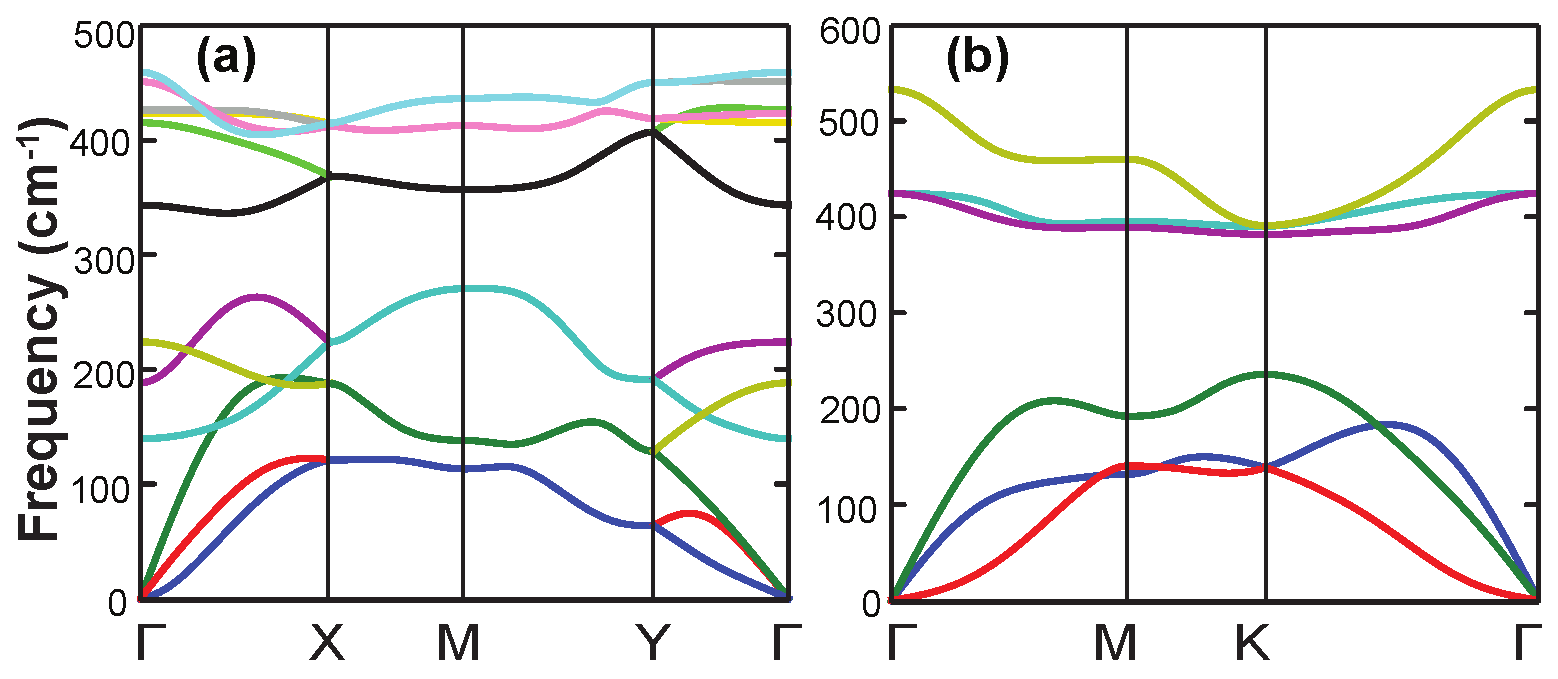
\includegraphics[width=0.8\linewidth]{phos_phon.eps}%
\caption{Calculated phonon dispersions for prinstine (a) black and (b) blue P. (c) Optical phonon modes together with their frequencies (in units of cm$^{-1}$) at the $\Gamma$ point and irreducible representations for black P and blue P. (c) Optical phonon modes together with their frequencies (in units of cm$^{-1}$) at the $\Gamma$ point and irreducible representations for black P and blue P.\label{fig:ire_phos}}
\end{figure}

\begin{figure}[htbp]
\centering
\includegraphics[width=0.8\linewidth]{strain_vib.eps}%
\caption{ (Color online) Variation of the $\Gamma$ frequencies with strain: (a) zigzag and (b) armchair direction of black P and (c) blue P.  \label{fig:shift_phos} }
\end{figure}

With the knowledge of the space group and its character table it is possible to assign vibrational modes to each band at the $\Gamma$-point. A table of all optical modes together with its frequency and irreducible representation for both structures is presented in \autoref{fig:ire_phos}(c) for the strainless structures. In \autoref{fig:shift_phos}, we show the variation of these optical phonons at the $\Gamma$ point under uniaxial strain. Our calculations agree well with the results of Ref.~\cite{phonon-blackP-1}. The frequency shift by strain can be directly detected using Raman spectroscopy. 
Depending on the atomic motion of the modes, the magnitude and type of strain, we find that the dependence of the phonon frequency can be different for each mode. Especially, the higher energy optical modes under uniaxial strain, applied along the zigzag direction, exhibit a much larger variation, see \autoref{fig:shift_phos}(a). B$^2_{3g}$ mode of black P has a different behavior under tensile and compressive strains along the zigzag direction. Applying a tensile (compressive) strain increases (decreases) the frequency of B$^2_{3g}$ mode. The frequency spacing between A$^2_{g}$ and B$_{2u}$ modes decreases when black P is stretched along both zigzag and armchair directions. While  the frequency of A$^2_{g}$ mode exhibits almost no variation under strain applied along the armchair direction,  it significantly varies under  strain applied along the zigzag direction.
Among the low lying optical modes (i.e., B$_{1u}$, B$_{1g}$ and B$^1_{3g}$), the B$_{1u}$ mode exhibits a larger variation with applied strain. 
E$_g$ and A$_{1g}$ modes of blue P always are red shifted when changing strain from compressive to tensile. Our results show that by measuring the frequency shift in the particular modes, it is possible to determine the
strain distribution in phosphorene.  

Our results show that the frequency shift observed in particular modes can be utilized to determine strain distribution in phosphorene.

\subsection[Carrier mobility enhancement in TiS$_3$ monolayer with strain]{Carrier mobility enhancement in TiS$_3$ monolayer with strain \footcite[This work is published in:][]{Aierken2016.mobility}}

%\subsection{Monolayer TiS$_3$}
%
%Bulk TiS$_3$ has a layered structure that makes it possible to exfoliate its monolayer. Indeed, such a process has been carried out by \citet{ADOM:ADOM201400043,ADMA:ADMA201405632} and results in the successful synthesis of a new type of 2D materials: monolayer TiS$_3$. The atomic structure of TiS$_3$ monolayer is shown in Fig.~\ref{structure}. The unit cell has a monoclinic crystal structure. The calculated lattice constants  are \textit{a} =  5.03 ~{\AA} and \textit{b} = 3.41~{\AA}, in good agreement with previous calculations \cite{Kang2015,Jin2015} and close to the experimental values for the bulk structure ($a$=4.958, $b$=3.401)\cite{Furuseth1975}. The monolayer is composed of connecting quasi-one-dimensional chains of TiS$_3$ triangular prisms extending along the \textit{b} direction, as shown in Fig.~\ref{structure}. One can spot a significant structural anisotropy in the system along the chain direction (green vector) and  the perpendicular direction (red vector).

\subsection{Carrier mobility}

\subsection[Magnetic properties modulation in penta-hexa-graphnene with strain]{Magnetic properties modulation in penta-hexa-graphnene with strain \footcite[This work is published in:][]{Aierken2016.magnetism}}

This new material has an antiferromagnetic (AFM) ground state which transforms to a ferromagnetic (FM) state under strain. The latter state is protected by a small strain-induced energy barrier. These findings can initiate further research to induce magnetism and spin-flip barriers through strain in other metal-free 2D materials.

\begin{figure}[htbp]
\centering
\includegraphics[width=\linewidth]{FM_AFM.eps}%   
\caption{AFM to FM transition of monolayer ph-graphene under strain. \label{transition}}
\end{figure}

Strain is an effective way to modulate the electronic properties of materials. \textcolor{red}{There are different ways to induce strain on 2D materials. \citet{Roldan2015} gave a comprehensive review on the strain engineering on 2D system both from experimental and theoretical view. }Here, we apply biaxial strain to our structure and monitor how the total energy of the different magnetic phases change, see \autoref{transition}. We find that an AFM to FM transition occurs for both compressive and tensile strains of approximately 6\% and 8\%, respectively. Therefore, strained structures of this kind can give a FM ground state, which is more beneficial for applications. The variation of the band gap under strain is plotted in \autoref{bandgap}. Both the FM and the AFM band gap has a similar qualitative behavior with a small quantitative difference between the two magnetic phases. The tensile strain decreases the band gap monotonically up to 10\%, while the compressive strain gives a non-monotonic behavior due to band crossings. From -5\% to 10\% strain, CBM and VBM are located at the $\Gamma$ and K high symmetric k-points, respectively. While two transitions of the location of the VBM happen below -5\% strain. First, it is shifted to the $\Gamma$ k-point from the second highest valence band around -8\%, and then shifted to the $\Sigma$ k-path between the $\Gamma$ and M k-points at -9\%.

\begin{figure}[htbp]
\centering
\includegraphics[width=\linewidth]{FM_AFM_Eg.eps}%   
\caption{ (Color online) Band gap variation of AFM and FM monolayer ph-graphene under strain. \label{bandgap}}
\end{figure}
\begin{figure}[htbp]
\centering
\includegraphics[width=\linewidth]{AFM_AFM_barrier.eps}%   
\caption{ (Color online) AFM to FM transition through spin-flip in monolayer ph-graphene. \label{spinflip} }
\end{figure}

As a final property of the two different magnetic ground states, we study the energy barrier for the transition from the FM to AFM state through spin flipping. This calculation is realized by constraining the magnetic moment through a penalty contribution to the total energy in VASP, and rotate one of the moments stepwise through 180$^{\circ}$.  In this way an energy profile from FM to AFM can be obtained (see \autoref{spinflip}). The rotation of the magnetic moment was carried along two different planes, one along the zigzag direction and the other along armchair direction, but the difference of the energy profile is negligible. Without strain, there is almost no energy barrier for the transition from the FM to AFM state. However, if the structure is under a 9\% tensile strain, in which case the FM state is the ground state, an energy barrier of about 13 meV per magnetic atom arises to return to the AFM state. This is much larger as one consider the energy barrier from the AFM to the FM under the same strain, which is about 3.3 meV per magnetic atom. \textcolor{red}{This calculation is performed with the aim to study the stability of each magnetic state, and the possibility to form paramagnetic state even without thermal mothion. We found both magnetic state is stable, and there is no tendency to form non-collinear magnetic moment orientation, and possibility of paramagnetic formation is small.}

We discovered a strain-driven magnetic ground state transition from AFM to FM around  6\% compressive strain and 8\% tensile strain. An energy profile with different angles between two local magnetic moments is calculated to study the energy barrier for the transition between FM and AFM. While an energy barrier of about 13 meV/(magnetic atom) protecting the AFM ground state in the pristine case; it is protecting the FM ground state when the system is under 9\% tensile strain.  

\section{Adatom adsorption}
\subsection[Nitrogen edge-decorated graphene nanoribbon]{Nitrogen edge-decorated graphene nanoribbon \footcite[This work will be published as:][]{Aierken2017.GNR}}

\section{Heterostructures}
\subsection[Electrical transport in 1T/2H/1T MoS2 lateral heterostructure]{Electrical transport in 1T/2H/1T MoS2 lateral heterostructure \footcite[This work is submitted as:][]{Aierken2017.transport}}
\subsection[Li storage and diffusion in MXenes/graphene vertial heterostructure]{Li storage and diffusion in MXenes/graphene vertial heterostructure \footcite[This work will be published as:][]{Aierken2017.battery}}

\section{Defect induction}
\subsection[Faceted blue phosphorene nanotube formed by line defects]{Faceted blue phosphorene nanotube formed by line defects \footcite[This work is published in:][]{Aierken2015.nanotubes}}
\subsection[Electronic structure of penta-hexa defects in graphene]{Electronic structure of penta-hexa defects in graphene \footcite[This work is published in:][]{Aierken2016.magnetism}}